% Source for the figure of CanonicalHuffman (sec. 21.2): the canonical code
% of the lengths a 4, b 4, c 3, d 2, e 2, f 3, g 3 as a tree skewed to the
% left, and the arrays fc and symb that the decoder reads instead of it.
% Build: make figures (in ../build).
\documentclass[border=4pt]{standalone}
\usepackage[T1]{fontenc}
\usepackage{newpxtext,newpxmath}
\usepackage[varqu,varl,scaled=0.95]{zi4}
\usepackage{tikz}
% tikz-ads.tex: the TikZ styles shared by the figures of the memory of the
% manual, \input by each standalone figure: a cell of a vector (cell), the
% cell that an operation touches (touched), a free cell (free), a node of a
% linked structure (node), the labels of indices (index) and of variables
% (var), a pointer (ptr), and \cells and \indices to draw a row of cells.
\usetikzlibrary{arrows.meta,positioning,calc,fit,shapes.multipart}
\definecolor{adsTouched}{RGB}{214,196,236}
\definecolor{adsFree}{RGB}{236,236,236}
\tikzset{
  ads/.style={>={Stealth[length=2mm]},font=\small,
              every node/.append style={inner sep=0pt}},
  cell/.style={draw,minimum width=7mm,minimum height=7mm,
               font=\small\ttfamily,outer sep=0pt},
  touched/.style={cell,fill=adsTouched},
  free/.style={cell,fill=adsFree,text=black!45},
  node/.style={draw,rounded corners=1pt,minimum width=8mm,
               minimum height=6mm,font=\small\ttfamily},
  index/.style={font=\scriptsize\ttfamily,text=black!60},
  var/.style={font=\small\itshape},
  ptr/.style={->,thick}
}
% \cells{name}{x,y}{list}: a row of cells, the first at (x,y), named
% name-0, name-1, ...; each item is text/style, the style one of cell,
% touched and free (e.g., {a/cell,e/touched,/free})
\newcommand{\cells}[3]{%
  \foreach \v/\s [count=\i from 0] in {#3}
    \node[\s] (#1-\i) at ($(#2)+(\i*7mm,0)$) {\v};}
% \indices{name}{n}: the indices 0 .. n-1 under the cells of name
\newcommand{\indices}[2]{%
  \foreach \i in {0,...,\numexpr#2-1\relax}
    \node[index,below=1.2mm of #1-\i] {\i};}

\begin{document}
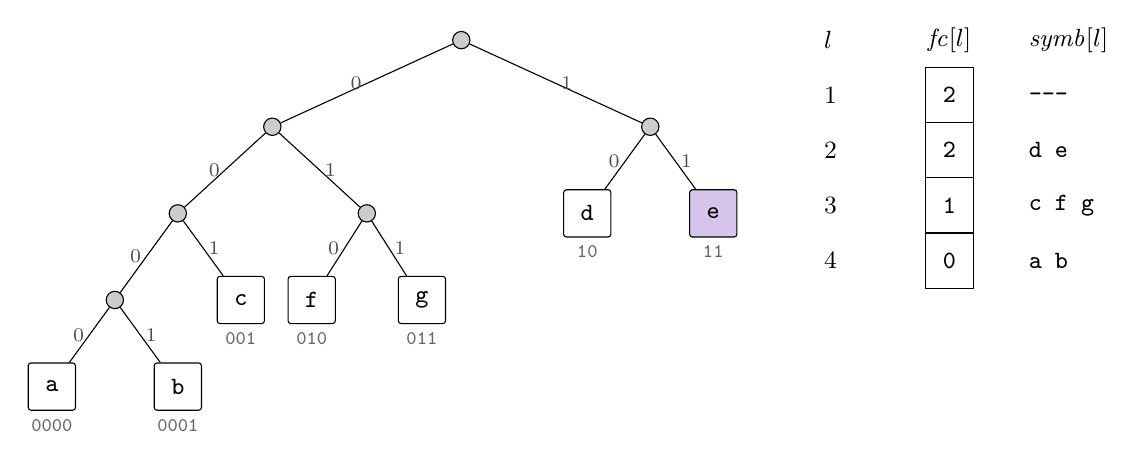
\begin{tikzpicture}[ads,
    inn/.style={draw,circle,minimum size=2.2mm,fill=black!20},
    lf/.style={node,minimum width=6mm},
    bit/.style={font=\scriptsize,text=black!70}]
  \node[inn] (r) at (0,0) {};
  \node[inn] (x) at (-24mm,-11mm) {};
  \node[inn] (y) at (24mm,-11mm) {};
  \node[inn] (x0) at (-36mm,-22mm) {};
  \node[inn] (x1) at (-12mm,-22mm) {};
  \node[lf] (d) at (16mm,-22mm) {d};
  \node[lf,fill=adsTouched] (e) at (32mm,-22mm) {e};
  \node[inn] (x00) at (-44mm,-33mm) {};
  \node[lf] (c) at (-28mm,-33mm) {c};
  \node[lf] (f) at (-19mm,-33mm) {f};
  \node[lf] (g) at (-5mm,-33mm) {g};
  \node[lf] (a) at (-52mm,-44mm) {a};
  \node[lf] (b) at (-36mm,-44mm) {b};
  \foreach \u/\v/\b/\s in {r/x/0/left,r/y/1/right,x/x0/0/left,x/x1/1/right,
      y/d/0/left,y/e/1/right,x0/x00/0/left,x0/c/1/right,x1/f/0/left,
      x1/g/1/right,x00/a/0/left,x00/b/1/right}
    \draw (\u) -- node[bit,\s=0.6mm] {\b} (\v);
  \foreach \v/\c in {a/0000,b/0001,c/001,f/010,g/011,d/10,e/11}
    \node[index,below=1mm of \v] {\c};
  % the arrays of the decoder
  \node[var,anchor=west] at (46mm,0) {$l$};
  \node[var] at (62mm,0) {$\mathit{fc}[ l ]$};
  \node[var,anchor=west] at (72mm,0) {$\mathit{symb}[ l ]$};
  \foreach \l/\f/\s [count=\k] in {1/2/{---},2/2/{d e},3/1/{c f g},4/0/{a b}}
    {\node[anchor=west] at (46mm,-\k*7mm) {\l};
     \node[cell,minimum width=6mm] at (62mm,-\k*7mm) {\f};
     \node[anchor=west,font=\small\ttfamily] at (72mm,-\k*7mm) {\s};}
\end{tikzpicture}
\end{document}
